%1. Describe EKS cluster
%2. Describe how was operator installed (screenshots etc)
%3. Describe prepared CRD
%4. Describe execution (screenshots)
%4.1 Aligning
%4.2 Prediction
%4.3 Post Processing
%5. Describe artifacts
%6. Show SMS

\chapter{Methods and Experiments}

This chapter aims to describe the evaluation methods of the KubeFold platform on the AWS cloud and discuss the computation results.

\section{Runtime environment}

The project was run on the AWS EKS platform~\ref{subsec:aws-eks}.
The \texttt{eksctl} tool was used to quickly launch the cluster, with the cluster configured in the \texttt{eu-central-1} region with two node groups - CPU and GPU.
The configuration is shown in listing~\ref{lst:eksctl}.
It's worth noting the attached AWS IAM policies that grant permissions for node groups to services such as AWS S3, AWS SNS, and AWS FSx.

\begin{lstlisting}[language=yaml,caption={\texttt{eksctl} configuration used for launching AWS EKS cluster},label={lst:eksctl}]
apiVersion: eksctl.io/v1alpha5
kind: ClusterConfig
metadata:
  name: alphafold-cluster
  region: eu-central-1

managedNodeGroups:
  - name: ng-primary # Cheaper node group without GPU devices
    instanceType: m5.xlarge
    desiredCapacity: 1
    subnets:
      - "subnet-038b10f6f4ac5aacd"
    iam:
      withAddonPolicies:
        ebs: true
        fsx: true
        efs: true
      attachPolicyARNs:
        - arn:aws:iam::aws:policy/AmazonEKSWorkerNodePolicy
        - arn:aws:iam::aws:policy/AmazonEKS_CNI_Policy
        - arn:aws:iam::aws:policy/AmazonFSxFullAccess
        - arn:aws:iam::aws:policy/AmazonS3FullAccess
        - arn:aws:iam::aws:policy/AmazonSNSFullAccess
        - arn:aws:iam::aws:policy/AmazonEC2ContainerRegistryReadOnly
        - arn:aws:iam::aws:policy/AmazonSSMManagedInstanceCore
  - name: ng-gpu # More expensive node group with GPU devices
    instanceType: g5.xlarge
    desiredCapacity: 1
    subnets:
      - "subnet-038b10f6f4ac5aacd"
    iam:
      withAddonPolicies:
        ebs: true
        fsx: true
        efs: true
      attachPolicyARNs:
        - arn:aws:iam::aws:policy/AmazonEKSWorkerNodePolicy
        - arn:aws:iam::aws:policy/AmazonEKS_CNI_Policy
        - arn:aws:iam::aws:policy/AmazonFSxFullAccess
        - arn:aws:iam::aws:policy/AmazonS3FullAccess
        - arn:aws:iam::aws:policy/AmazonSNSFullAccess
        - arn:aws:iam::aws:policy/AmazonEC2ContainerRegistryReadOnly
        - arn:aws:iam::aws:policy/AmazonSSMManagedInstanceCore

iam:
  withOIDC: true
  serviceAccounts:
    - metadata:
        name: fsx-csi-controller-sa
        namespace: kube-system
        labels: { aws-usage: "application" }
      attachPolicyARNs:
        - "arn:aws:iam::aws:policy/AmazonFSxFullAccess"

vpc:
  id: vpc-0ade33da149682ec2
  subnets:
    public:
      eu-central-1a:
        id: "subnet-038b10f6f4ac5aacd"
      eu-central-1b:
        id: "subnet-099b2b55ca156bb7d"

addons:
  - name: vpc-cni
  - name: coredns
  - name: kube-proxy
  - name: eks-pod-identity-agent
\end{lstlisting}

On the cluster, the AWS FSx CSI Driver has been installed.
It is used for automatic creation and management of AWS FSx for Lustre volumes based on \texttt{PersistentVolumeClaim} resources created in the cluster.
To make this possible, it is necessary to configure a \texttt{StorageClass} that specifies how volumes should be created.
In the configuration shown in listing~\ref{lst:storage-class}, parameters such as file system version, compression type (disabled), volume throughput, and network settings were defined.
This means that creating a \texttt{PersistentVolumeClaim} resource pointing to the \texttt{StorageClass} named \texttt{fsx-sc} will automatically provision a new FSx file system in AWS.

\begin{lstlisting}[language=yaml,caption={Definition of \texttt{StorageClass} for FSx CSI Driver},label={lst:storage-class}]
kind: StorageClass
apiVersion: storage.k8s.io/v1
metadata:
  name: fsx-sc
provisioner: fsx.csi.aws.com
parameters:
  subnetId: subnet-038b10f6f4ac5aacd
  securityGroupIds: sg-058c31d84bfd004cf,sg-04e79090b86912eae,sg-07d7ceb3fa050568c,sg-02a2a067c7f724318
  deploymentType: PERSISTENT_1
  perUnitStorageThroughput: "200"
  dataCompressionType: "NONE"
  fileSystemTypeVersion: "2.15"
\end{lstlisting}

The KubeFold operator was installed using the installation file generated by the KubeBuilder tool.
It is located in the GitHub code repository under the path \texttt{dist/install.yaml}.
The installation therefore comes down to executing a single command: \texttt{kubectl apply -f https://raw.githubusercontent.com/kubefold/operator/ \n refs/heads/main/dist/install.yaml}.
This makes it very fast and convenient from the administrator's perspective.

\begin{lstlisting}[language=bash,caption={Quick project startup script},label={lst:up-script}]
#!/bin/bash

export AWS_PAGER=""
ACCOUNT_ID=$(aws sts get-caller-identity --query Account --output text)
eksctl create cluster -f eks/cluster.yaml
aws eks update-kubeconfig --name alphafold-cluster --region eu-central-1
kubectl config use-context arn:aws:eks:eu-central-1:"$ACCOUNT_ID":cluster/alphafold-cluster
kubectl apply -k "github.com/kubernetes-sigs/aws-fsx-csi-driver/deploy/kubernetes/overlays/stable/?ref=release-1.3"
kubectl apply -f eks/fsx.storageclass.k8s.yaml

kubectl apply -f https://raw.githubusercontent.com/kubefold/operator/refs/heads/main/dist/install.yaml
kubectl apply -f config/samples/data_v1_proteindatabase.yaml

echo 'Done'
\end{lstlisting}

A \texttt{up.sh} script was prepared for quickly setting up the environment with all necessary dependencies, which is shown in listing~\ref{lst:up-script}.
After executing the script, you can directly proceed to start working with KubeFold.
If the setup was installed correctly, running the command \texttt{kubectl get pods -A} should show output similar to that in screenshot~\ref{fig:eks_pods_terminal}.

\begin{figure}[htbp]
    \centering
    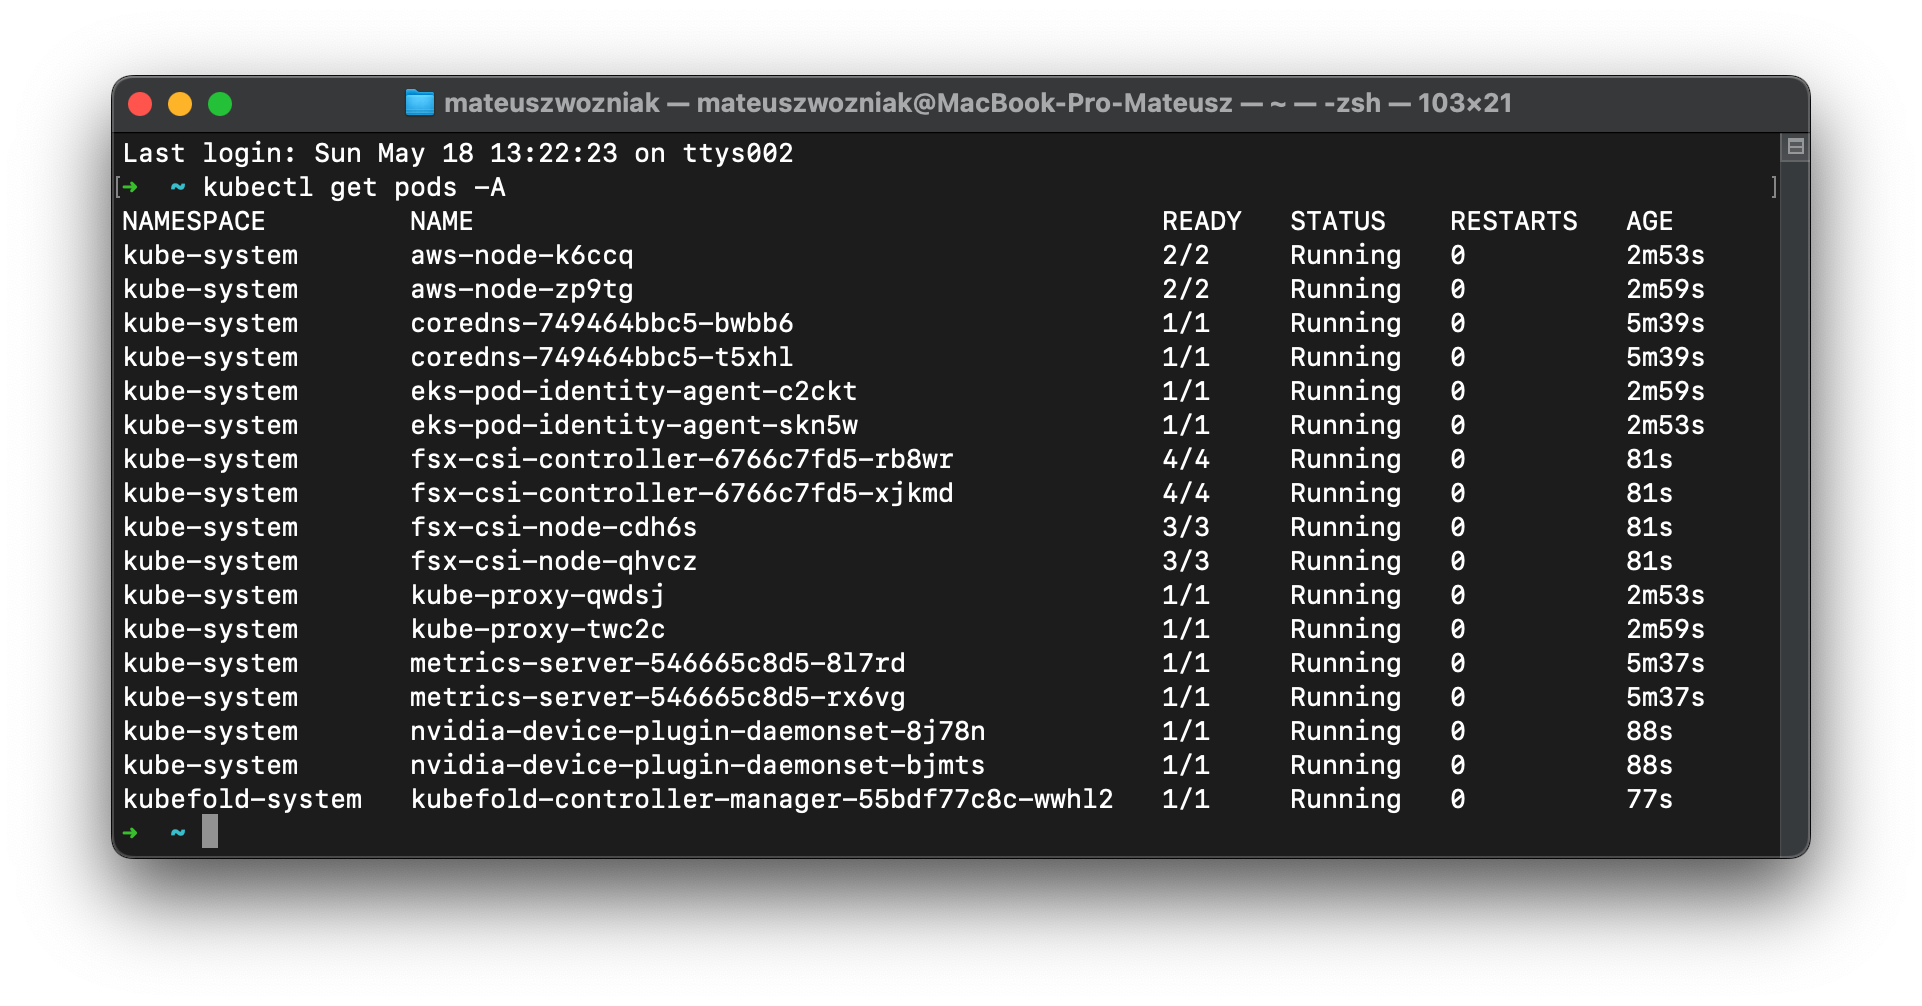
\includegraphics[width=\textwidth]{images/eks_pods_terminal}
    \caption{\texttt{kubectl get pods} output after successful cluster installation}
    \label{fig:eks_pods_terminal}
\end{figure}

\section{Prepared resource definitions}

The following YAML resource definitions were prepared for testing KubeFold.
The first one is the \texttt{ProteinDatabase} resource shown in listing~\ref{lst:used_protein_database}.
The second one is the \texttt{ProteinConformationPrediction} resource shown in listing~\ref{lst:used_protein_conformation_prediction}.
Both resources were applied to the cluster using \texttt{kubectl apply} right after installation.

\begin{lstlisting}[language=yaml,caption={Used \texttt{ProteinDatabase} resource definition},label={lst:used_protein_database}]
apiVersion: data.kubefold.io/v1
kind: ProteinDatabase
metadata:
  name: proteindatabase-sample
spec:
  datasets:
    bfd: true
    mgyclusters: true
    nt: true
    pdb: true
    pdbseqreq: true
    rfam: true
    rnacentral: true
    uniref90: true
    uniprot: true
  volume:
    storageClassName: fsx-sc
\end{lstlisting}

\begin{lstlisting}[language=yaml,caption={Used \texttt{ProteinConformationPrediction} resource definition},label={lst:used_protein_conformation_prediction}]
apiVersion: data.kubefold.io/v1
kind: ProteinConformationPrediction
metadata:
  name: proteinconformationprediction-sample
spec:
  database: proteindatabase-sample
  protein:
    id: [ 'A','B' ]
    sequence: GMRESY...LQQANDLKQG
  model:
    volume:
      storageClassName: fsx-sc
    weights:
      http: https://staticfilehosting.com/af3.bin.zst
    seeds:
      - 1
  destination:
    s3:
      bucket: kubefold-artifacts-sample
      region: eu-central-1
  notify:
    region: eu-central-1
    sms:
      - "+48140690323"
\end{lstlisting}.

When the \texttt{ProteinDatabase} resource was created, the FSx CSI Driver triggered the creation of an FSx for Lustre file system (see fig.~\ref{fig:fsx_fs}).
As soon as the file system was created, the process of downloading protein databases began in multiple pods simultaneously.
The user can monitor the download progress in real-time, as shown in screenshot~\ref{fig:used_proteindatabase_terminal}.
After the download is complete, the status will be changed to \textit{Completed} (see screenshot~\ref{fig:proteindatabase_completed_terminal}).

\begin{figure}[htbp]
    \centering
    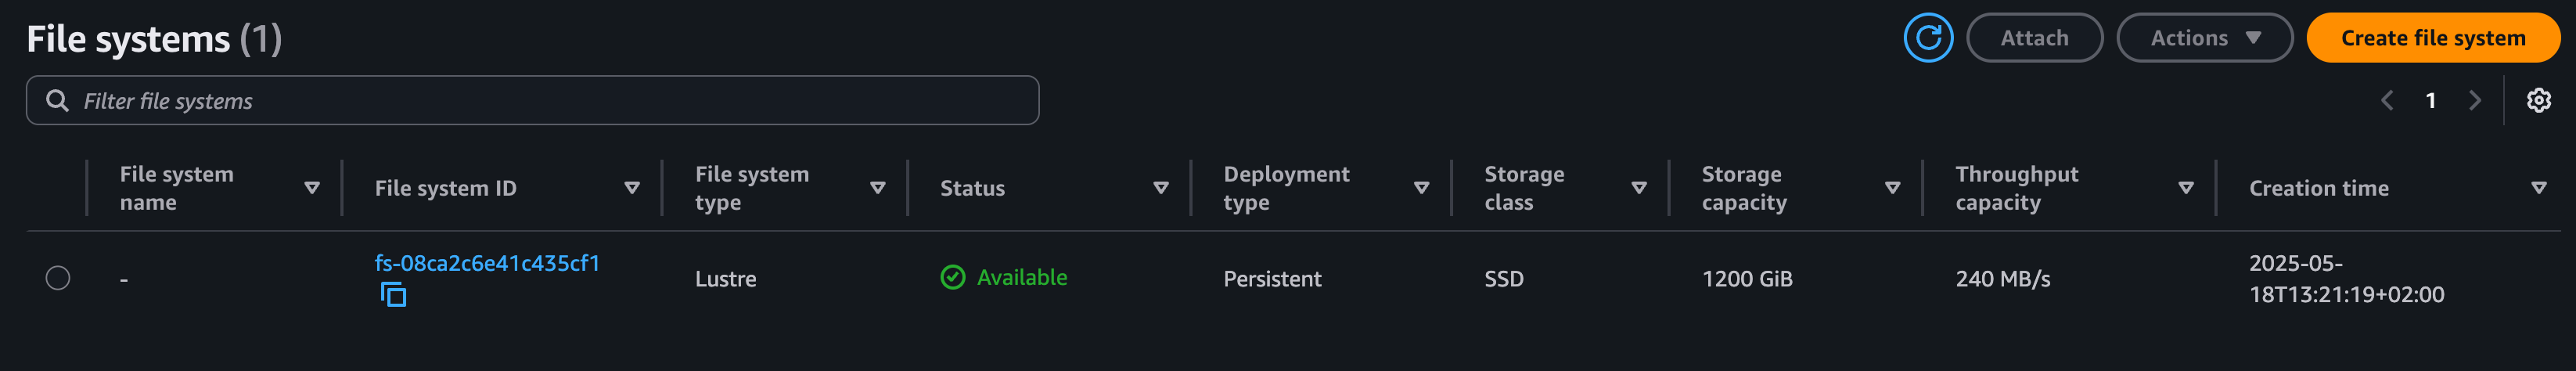
\includegraphics[width=\textwidth]{images/fsx_fs}
    \caption{Created FSx for Lustre file system in AWS Web Console}
    \label{fig:fsx_fs}
\end{figure}

\begin{figure}[htbp]
    \centering
    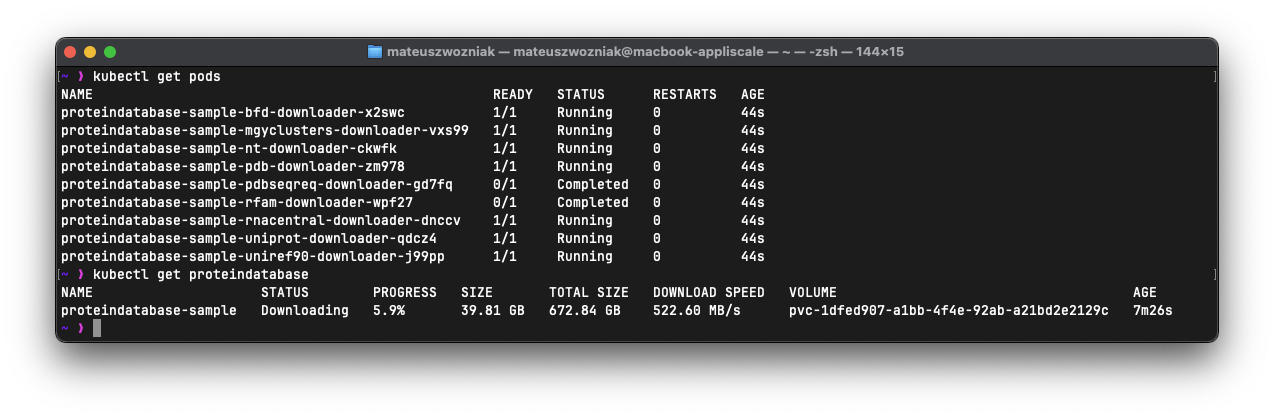
\includegraphics[width=\textwidth]{images/old_proteindatabase_terminal}
    \caption{Terminal output presenting \texttt{ProteinDatabase} resource}
    \label{fig:used_proteindatabase_terminal}
\end{figure}

\begin{figure}[htbp]
    \centering
    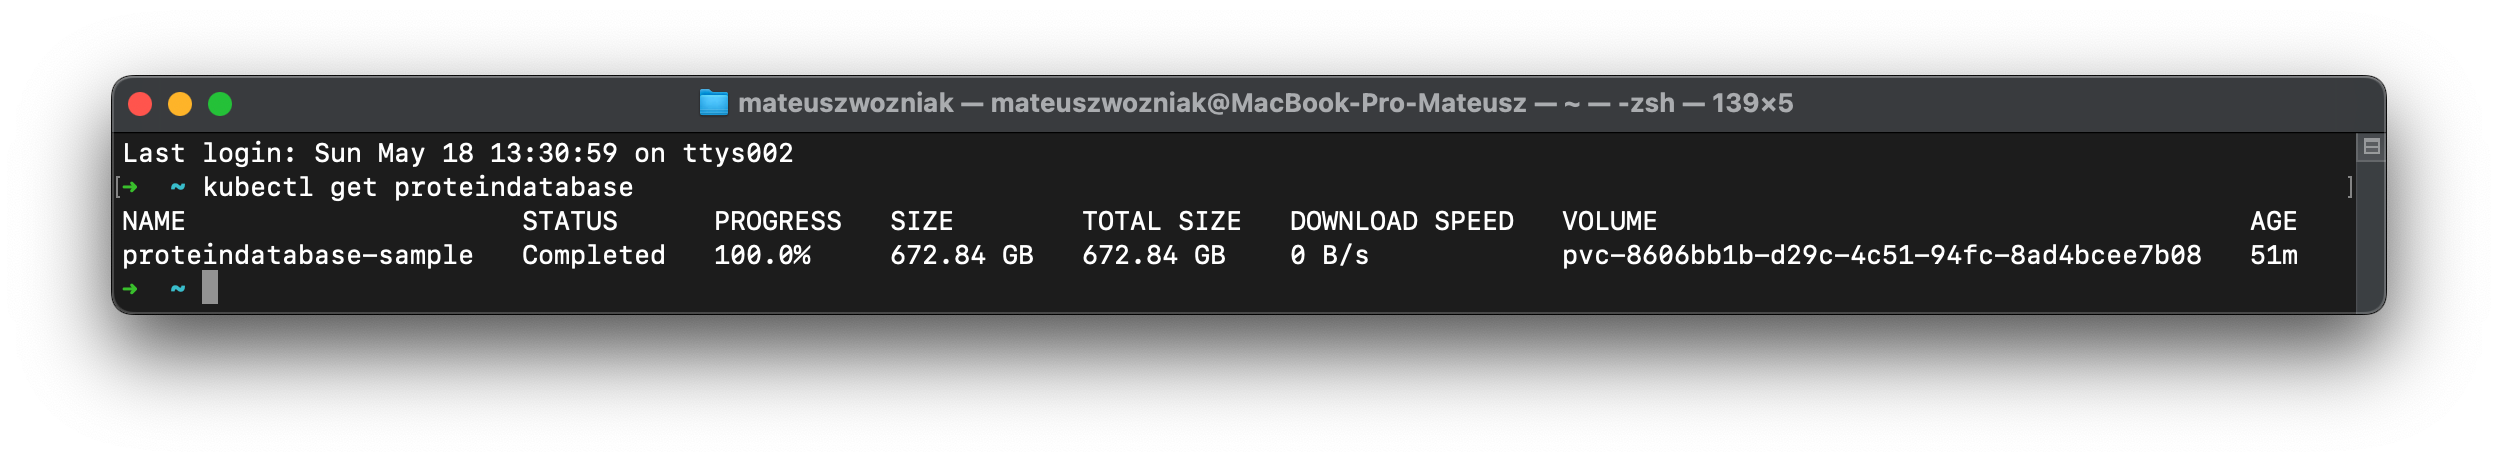
\includegraphics[width=\textwidth]{images/proteindatabase_completed_terminal}
    \caption{Completed downloading of protein database}
    \label{fig:proteindatabase_completed_terminal}
\end{figure}

After applying the \texttt{ProteinConformationPrediction} resource, the KubeFold operator launches three Jobs in sequence, corresponding to three phases of the task.
The initial phase is the \textit{Aligning} phase, which the user can check by running the \texttt{kubectl get proteinconformationprediction} command in the terminal (see screenshot~\ref{fig:proteinconformationprediction_aligning_terminal}). It launches a pod with the \texttt{-search} suffix on a node equipped with large CPU resources.

The second phase is the \textit{Predicting} phase (terminal output is shown in screenshot~\ref{fig:proteinconformationprediction_predicting_terminal}), which runs on a node equipped with a tensor computation accelerator such as GPU or TPU.
In this phase, the pod was created with the \texttt{-predict} suffix.

The final phase is the \texttt{UploadingArtifacts} phase, which is responsible for sending computation artifacts to AWS S3 storage and queuing notifications to research team members (see screenshot~\ref{fig:proteinconformationprediction_uploading_terminal}). When this step is completed, the status will be changed to \texttt{Completed} (see screenshot~\ref{fig:proteindatabase_completed_terminal}).

\begin{figure}[htbp]
    \centering
    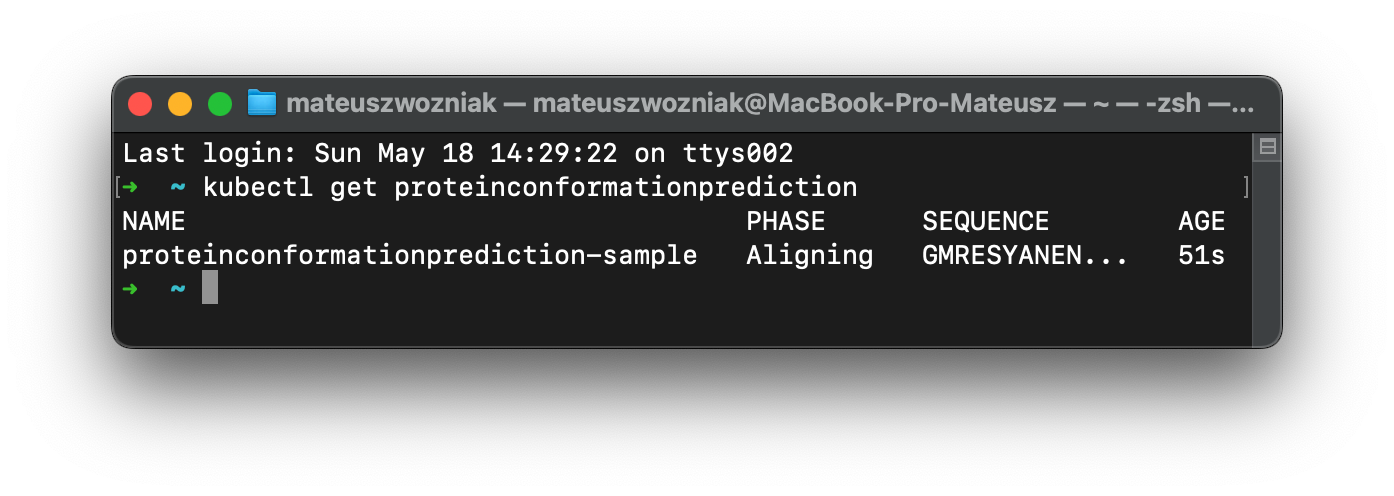
\includegraphics[width=\textwidth]{images/proteinconformationprediction_aligning_terminal}
    \caption{Aligning phase in protein conformation prediction task}
    \label{fig:proteinconformationprediction_aligning_terminal}
\end{figure}

\begin{figure}[htbp]
    \centering
    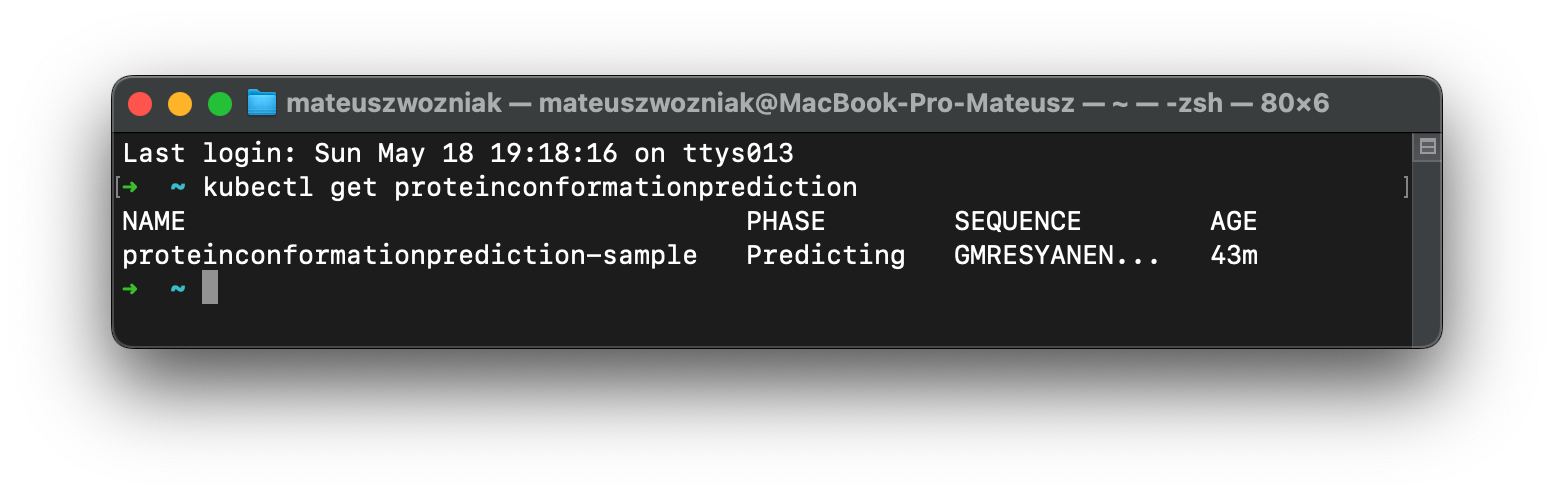
\includegraphics[width=\textwidth]{images/proteinconformationprediction_predicting_terminal}
    \caption{Predicting phase in protein conformation prediction task}
    \label{fig:proteinconformationprediction_predicting_terminal}
\end{figure}

\begin{figure}[htbp]
    \centering
    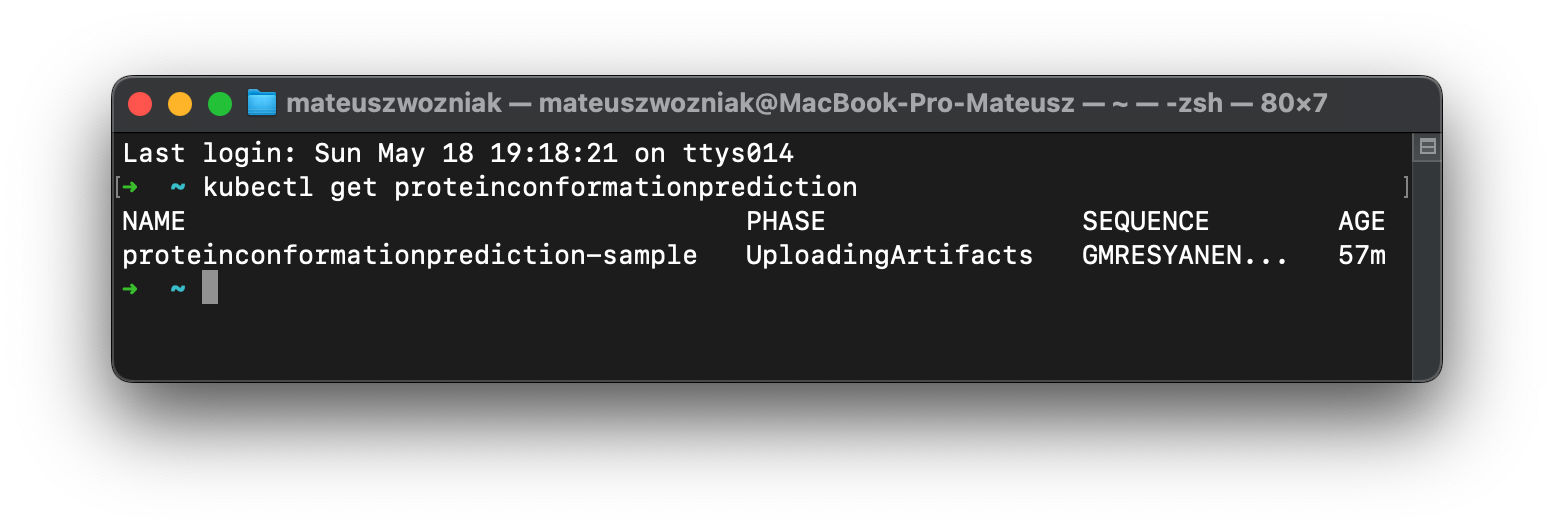
\includegraphics[width=\textwidth]{images/proteinconformationprediction_uploading_terminal}
    \caption{Post processing phase in protein conformation prediction task}
    \label{fig:proteinconformationprediction_uploading_terminal}
\end{figure}

\begin{figure}[htbp]
    \centering
    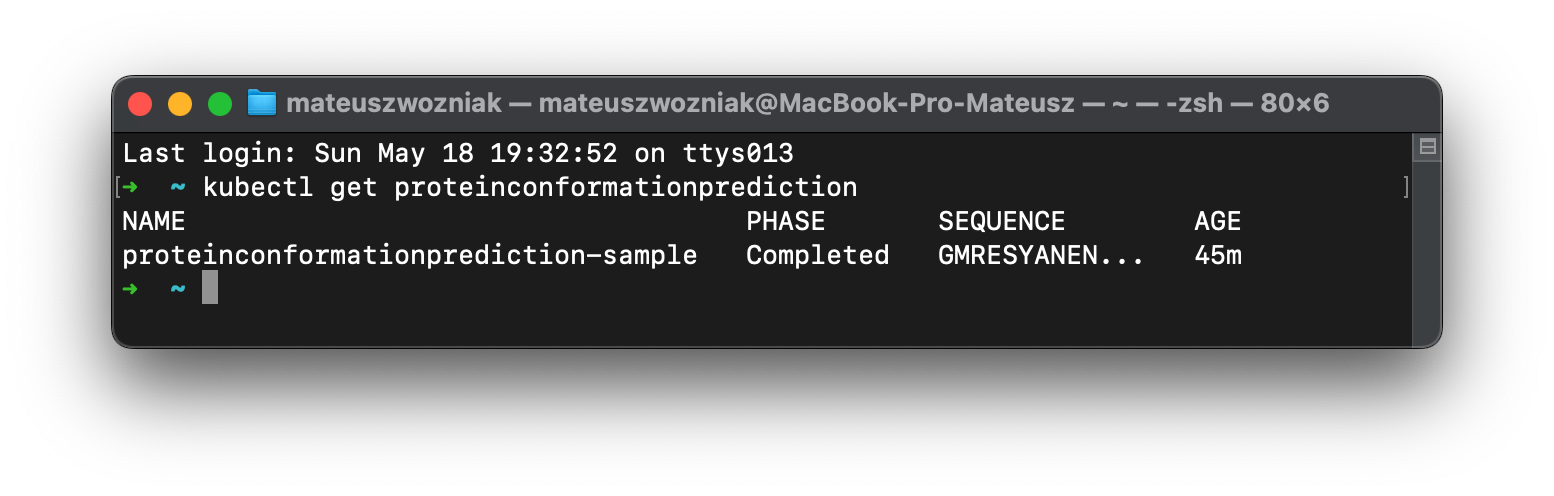
\includegraphics[width=\textwidth]{images/proteinconformationprediction_completed_terminal}
    \caption{Completed protein conformation prediction task}
    \label{fig:proteinconformationprediction_completed_terminal}
\end{figure}

\section{Computation artifacts overview}

After the computations were completed, the artifacts were sent to AWS S3 storage.
A directory was created in the bucket with a name containing the computation execution time, e.g., \texttt{default-proteinconformationprediction-sample\_20250518\_181911}.
The name also includes the Kubernetes resource name and namespace.
The directory contents are shown in screenshot~\ref{fig:bucket}.
%TODO(matisiekpl): discuss each file

The \texttt{.cif} file allows visualization of the three-dimensional protein structure using software such as \textit{RCSB 3D View} (\url{https://www.rcsb.org/3d-view}).
An example visualization is shown in fig.~\ref{fig:protein_visualization}.

Additionally, an SMS message was sent to the user informing about the completed computation (see fig.~\ref{fig:sns_notification}).

\begin{figure}[htbp]
    \centering
    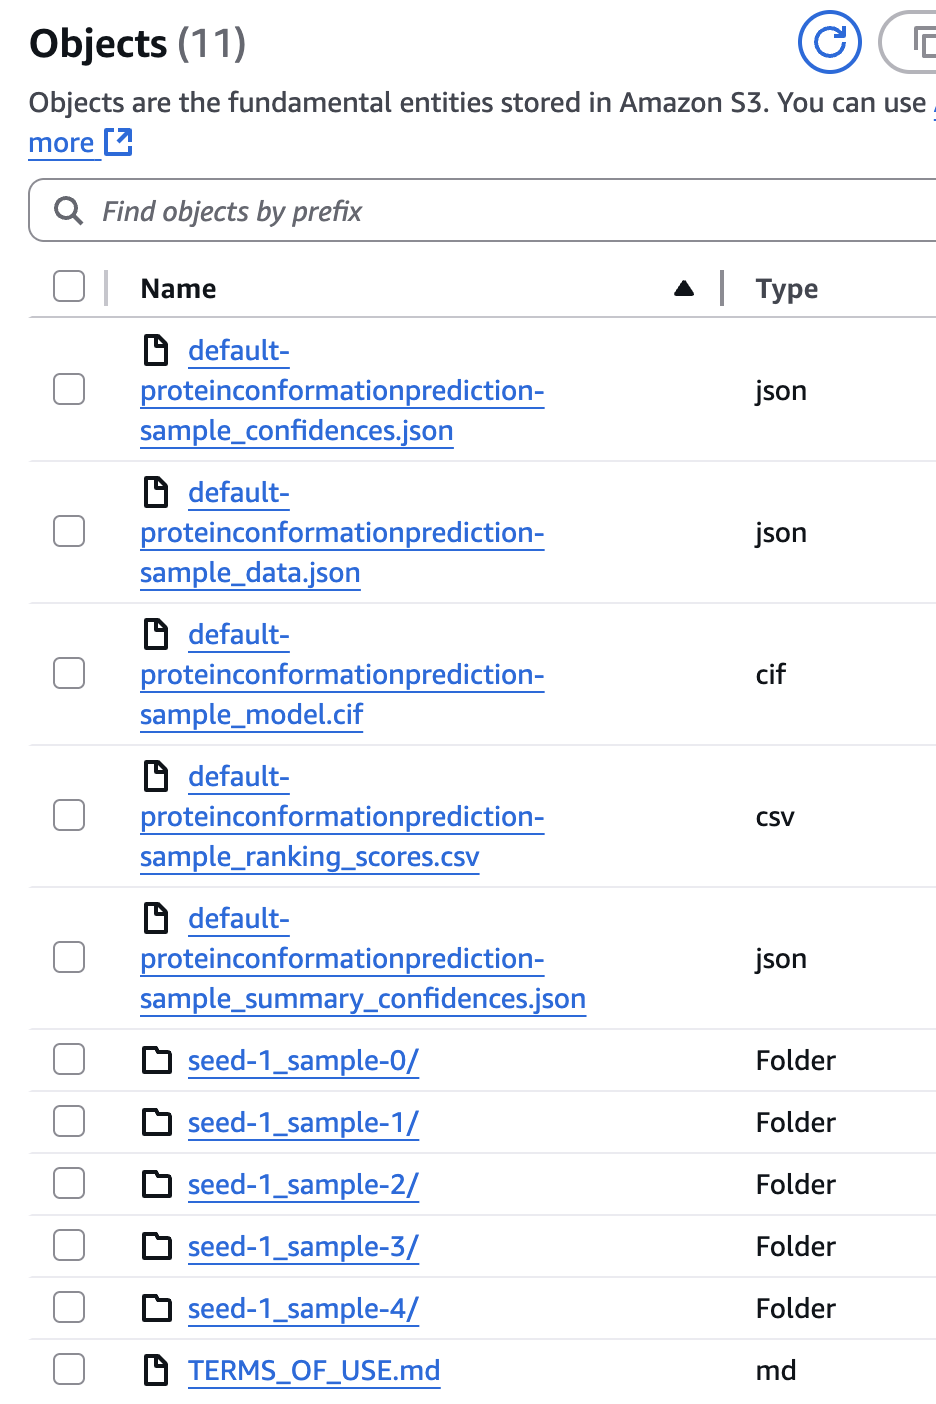
\includegraphics[width=\textwidth]{images/bucket2}
    \caption{Contents of bucket containg computation artifacts}
    \label{fig:bucket}
\end{figure}

\begin{figure}[htbp]
    \centering
    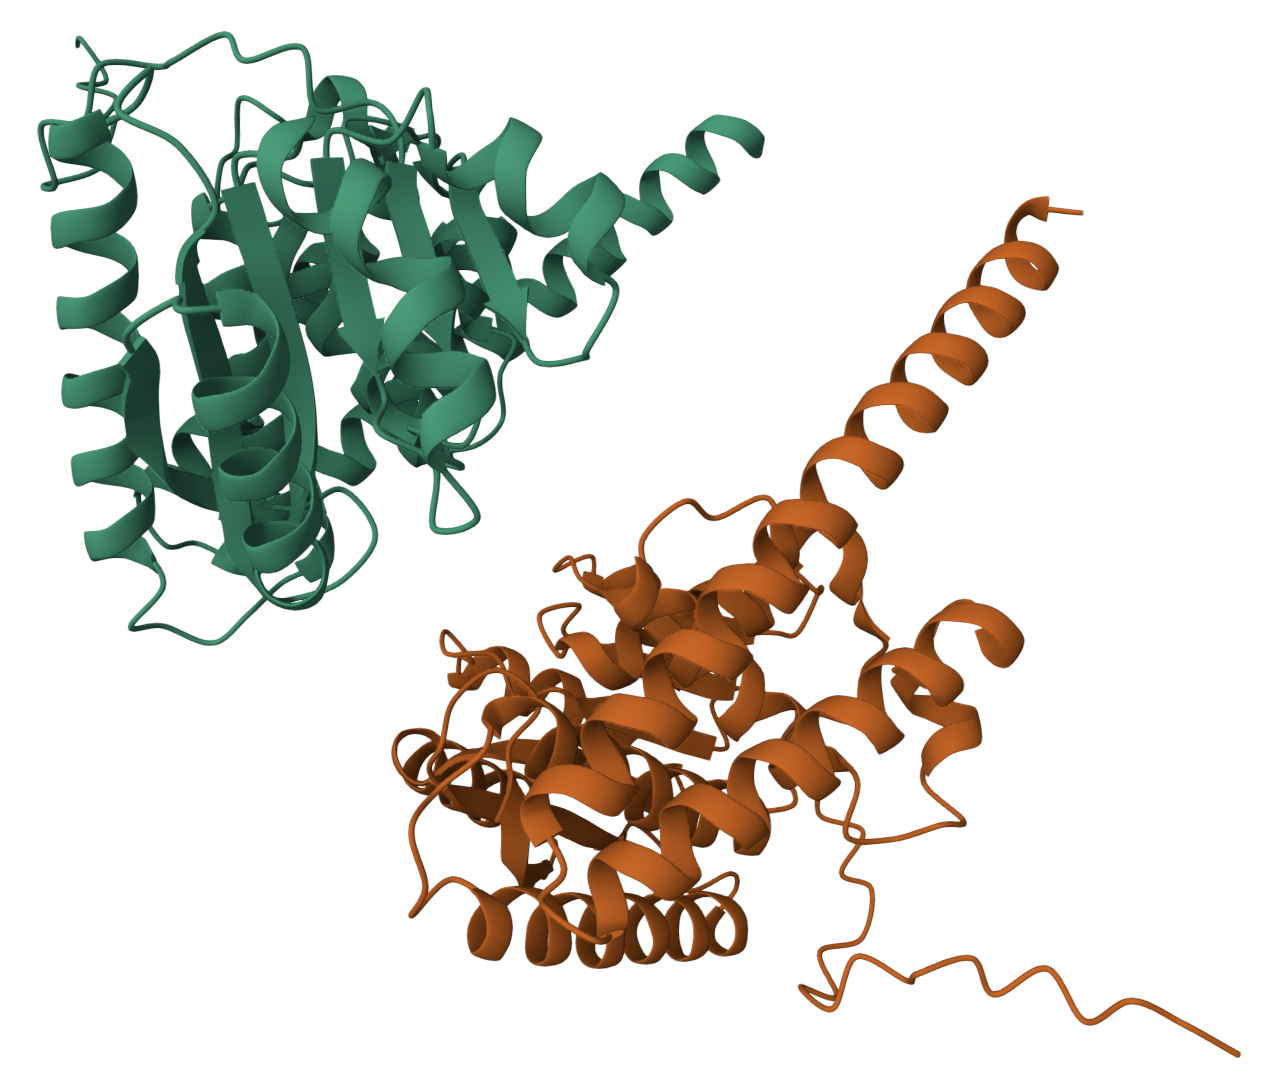
\includegraphics[width=\textwidth]{images/protein_visualization_small}
    \caption{Visualization of folded protein using RCSB visualization software \url{https://www.rcsb.org/3d-view}}
    \label{fig:protein_visualization}
\end{figure}

\begin{figure}[htbp]
    \centering
    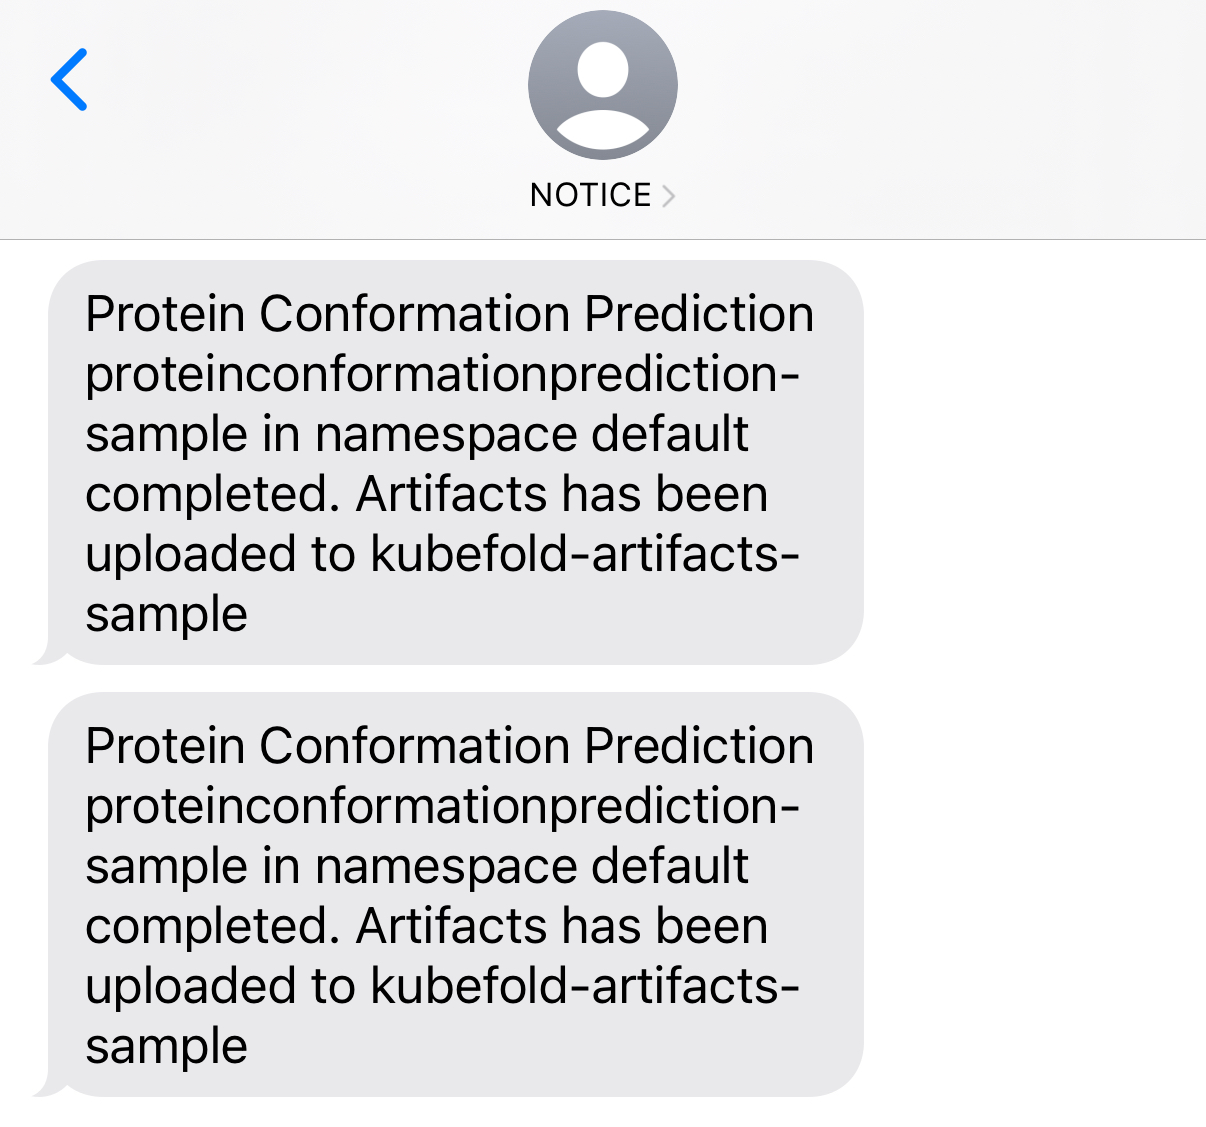
\includegraphics[width=\textwidth]{images/sns_notification_light}
    \caption{SMS Notification sent to research team member when computation is done}
    \label{fig:sns_notification}
\end{figure}
